\chapter{运行相变：探索、执行与结构更新的临界控制}
\label{chp:phase_transition_meta}

智能系统不会始终以同一种方式运行：熟练任务需要稳定而低分支的执行，未知问题需要扩展候选和主动试探，持续失配又可能要求修改结构。把这些变化统称为温度、熵或临界性虽然直观，却容易把采样随机性、表示结构、控制增益、资源负载和物理能耗混成一个量。本章把“相变”限定为可观测运行统计随控制参数变化而发生的定性重组。我们先定义任务相关序参量，再区分稳定执行、无序搜索和自适应临界区间；随后讨论宏观控制器如何调节探索并提交结构更新，为什么LLM末端采样温度不是系统温度，以及何种证据才足以支持涌现判断。物理相变提供模型工具而不是机制证明；HSF-HD给出一般状态动力学，AgentOS中的SPC、TCE与CCM只是其中一种可执行实现。

\section{任务相关序参量：结构复杂度、传播范围与目标对齐}
\label{sec:section_6298}

序参量的作用，是把无法逐项追踪的高维运行状态压缩成可比较的宏观读出，而不是量化所谓“灵魂”。设时刻 $t$ 的联合状态为 $z_t=(h_t,s_t,b_t,r_t)$：$h_t\in\mathbb R^d$ 是快速活动状态，$s_t=(G_t,\Theta_t)$ 是带版本的局部结构网络，$b_t$ 是对环境和候选策略的全局分布表示，$r_t$ 是资源账本。任务规范 $q_t$ 给出查询族、时间窗、容许误差与硬约束。我们定义序参量向量
\[
 m_t=P_{q_t,W}(z_{t-W:t})=(S_t,C_t,A_t,L_t,R_t),
\]
其中 $W$ 是观测窗；$S_t$ 描述任务相关结构复杂度，$C_t$ 描述扰动传播与恢复，$A_t$ 描述动作对目标的对齐，$L_t$ 描述负载和拥塞，$R_t$ 描述结构周转。投影 $P$ 的任务、窗口、归一尺度和数据来源都是定义的一部分。同一系统换任务或换窗口时，序参量可改变，因此不存在脱离测量协议的普遍“智能温度计”。

旧稿的图谱熵密度可以保留为结构读出，但需要修正其解释。对固定时间窗内的无向加权图 $G_t=(V_t,E_t,W_t)$，令归一化拉普拉斯为 $L_t=I-D_t^{-1/2}W_tD_t^{-1/2}$，非负特征值为 $\lambda_i$。若 $\sum_i\lambda_i>0$，定义 $p_i=\lambda_i/\sum_j\lambda_j$ 与
\[
 S_{spec}(G_t)=-\frac{1}{\log n_t}\sum_{i=1}^{n_t}p_i\log p_i.
\]
它无量纲且落在声明范围内，但只描述所选图、权重和节点集的谱分散。低值不必然意味着偏执或晶体，高值也不必然意味着随机、幻觉或精神病；不同非同构图甚至可能同谱。若节点数和权重随时间变化，必须先定义对齐、重采样或谱测度距离。真正与任务有关的结构复杂度还应加入查询保持项，例如在边遮蔽、节点移除和权重扰动下，读出 $Q_q$ 的变化 $\Delta_q=\sup_{\delta\in\mathcal D}d(Q_q(G),Q_q(G+\delta))$。这样才能区分“谱很丰富但任务脆弱”和“谱较集中但任务稳健”。

旧稿的场连贯性 $\xi$ 可重建为传播范围和恢复尺度。令 $a_i(t)$ 是经身份对齐的节点活动，先扣除共同输入和基线，计算条件相关函数 $C_q(i,j;\tau)$。在固定图距离 $d_G$ 和局部平稳区间内，若经验包络可由 $c_0d^{-\alpha}\exp(-d/\xi)$ 合理拟合，则 $\xi$ 是该模型下的相关长度；拟合失败时不应强报一个数。相关不等于因果：共同广播可让远端节点同步，却不表示信息沿路径传播。我们因此补充扰动响应
\[
 C_t^{int}(r)=\mathbb E\left[d\bigl(Q_q(z_{t+\tau}^{do(i,\epsilon)}),Q_q(z_{t+\tau})\bigr)\mid d_G(i,j)=r\right]
\]
以及恢复时间 $\tau_{rec}$。传播范围变长既可能提高跨域整合，也可能放大错误级联；无限相关长度不是顿悟的定义，更不能由一次全局同步推出宏观量子态。

旧稿的规范极化度 $M$ 可改写为目标对齐度。对窗口内实际提交的动作 $u_k$，定义目标方向 $g_k=-\nabla_uJ_{q_k}$ 或离散可行改进集合，令
\[
 A_t=\frac{\sum_{k=t-W+1}^{t}w_k\langle u_k,g_k\rangle}
 {\sum_{k=t-W+1}^{t}w_k(\|u_k\|\|g_k\|+\epsilon)}.
\]
$A_t$只在动作与目标方向位于同一内积空间时成立。高对齐表示动作一致地追随当前目标，不表示目标正确；极端高值可能是刚性服从，低值可能来自多目标权衡、探索动作、执行器故障或目标版本冲突。故还要记录约束违例率、策略多样性、外部任务成绩和目标来源。企业所有员工都对齐KPI可能同时集体刷指标，这正是“意志统一”等于智能的反例。

结构复杂度、传播范围和目标对齐不能合成一个未经校准的总分。我们保留向量序参量，并在任务需要时用Pareto区域或带硬约束的分层判定。局部结构网络负责节点身份、关系、来源和权限；全局分布表示负责候选、置信度与不确定性；二者通过身份绑定、消息耦合和读出接口联合。AgentOS可以由SPC压缩 $h(t)$ 的任务状态，由CCM估计负载、循环和传播范围，由TCE调节控制增益；但一般智能系统可以采用其他观测器。序参量必须能由日志重算、随版本复现并对干预作出可预期响应，否则它只是富有感染力的命名。

从统计上识别运行区间，需要先建立基线而非凭单点阈值。我们在多个任务、随机种子和扰动强度上采集 $m_t$，估计条件分布 $p(m\mid q,c)$，再用变化点、迟滞环、双峰分布或临界减速等证据判断是否存在状态重组。仅看到幂律直线或熵值居中，不能证明自组织临界；有限样本、混合分布和测量截断都能制造相似外观。序参量在本章因此是可证伪的运行摘要：它帮助定位何时换控制策略，却不替代因果模型、外部验收和安全边界。

\section{运行相态：稳定执行、无序搜索与自适应临界区间}
\label{sec:section_6651}

我们把“晶体、气体与液体”保留为三类运行区间的辅助名称，不把它们当作智能载体的真实物态。系统的控制参数记为 $c_t=(\tau_t,g_t,\rho_t,b_t^{res})$：$\tau_t$ 是候选采样尺度，$g_t$ 是目标与抑制增益，$\rho_t$ 是结构更新率，$b_t^{res}$ 是资源预算。快状态 obey $h_{k+1}=F(h_k,s_k,o_k,u_k,\eta_k;c_k)$，慢结构由事务映射 $s_{k+1}=U(s_k,\mathcal E_k;c_k)$ 更新。相态是统计量 $m_t$ 在给定任务族中的稳定分区；当参数连续变化而占用分布、恢复时间或结构周转发生显著跃迁和迟滞时，我们才使用相变一词。

稳定执行区间对应旧稿的层流或晶体态。其典型特征是候选有效数低、策略切换少、目标对齐高、扰动增益有界、结构版本基本不变。对已经校准的算术、编译、熟练驾驶或重复工具调用，这种区间能降低时延并提高复现性。若固定结构和目标下存在Lyapunov函数 $V$，使
\[
 V(h_{k+1})-V(h_k)\le-\alpha\|e_k\|^2+\gamma\|w_k\|^2,
\]
则可得到局部输入到状态界，但这不等于“耗散最低”或零能耗。执行仍消耗计算资源和电能，稳定也不保证输出事实正确。其失效模式是刚性：面对分布外观测、目标变化或不可行约束时，系统继续复用旧轨迹。老司机在熟悉道路上高效，遇到道路塌方若仍沿旧路线行驶，就是稳定控制超出适用域。

无序搜索区间对应旧稿的气体或离子态。这里候选有效数、状态总变差和策略切换率升高，目标对齐下降，验证积压与资源占用上升。它不必是病理：头脑风暴、广域检索和故障排查早期都需要暂时扩大搜索。危险来自搜索与验收脱耦——生成速率超过验证速率时，候选在 $h(t)$ 中拥塞，来源绑定丢失，局部错误经共享通道级联。我们用无量纲负载
\[
 L_t=\frac{\lambda_{in}(t)\,\mathbb E[c_{verify}(t)]}{\mu_{verify}(t)+\epsilon}
\]
表示单位窗内输入到达和验证服务能力的比值。$L_t>1$持续存在提示队列发散风险，但它不是雷诺数，也不推出人的临床状态。对LLM，高采样温度可能增加词元多样性，却不必增加内部推理搜索，更不能把幻觉单独归因于“高温”。

自适应临界区间位于可重复执行与广域搜索之间：系统保持足够候选以逃离局部策略，又能用身份、约束和回执迅速筛除无效分支。其操作判据不是“关联长度无穷大”，而是在预算内同时满足四项条件：对小扰动有可测但有界的响应；任务收益对适度探索呈正增益；错误级联可在规定时间恢复；结构更新经保留测试后提高跨情境表现。我们可定义任务敏感度 $\chi_q=\partial\mathbb E[Y_q]/\partial a$，其中 $a$ 是受控扰动幅度；只有在明确区间内估计，不能外推到奇异发散。真正的系统若响应无界，往往意味着不稳定而非创造力。

洗澡时突然想到数学解的旧例，可以解释为后台重组、线索变化和候选读出的共同结果，不需要假设全脑瞬时锁相或调和零模。要检验“临界区间有利于洞见”，应预注册任务、控制练习时间和休息，记录候选数量、验证链、解决率与恢复时间，并与固定低探索和高探索基线比较。一次戏剧性顿悟不能证明相变；反过来，渐进式证明也同样是创造性成果。物理临界现象提供有关响应、尺度和涨落的数学语言，但人类经验只构成启发性证据。

相态之间通常存在迟滞和路径依赖。升高探索尺度从稳定执行进入搜索的阈值，不一定等于降低探索重新回到执行的阈值；结构在高探索期间被修改后，返回路径更会改变。我们以混合系统表示：连续状态在模式 $m\in\{execute,search,adapt\}$ 内演化，守卫条件触发模式切换，重置映射处理缓存、积分器、候选集和权限。每次切换必须记录原因、前后参数、未决动作和回滚点。否则频繁“调温”会产生抖振，系统在探索与执行间来回切换，反而浪费预算。

图像 \texttt{figure/p\_t.pdf} 仍应保留，但图中的轴必须解释为运行控制量而非真实压强和热力学温度。横轴可表示探索尺度或候选熵，纵轴可表示目标控制增益，区域边界由实验估计并带置信区间；不同任务和载体会得到不同边界。SPC可提供任务状态压缩，TCE可在相图上选择模式，CCM监视负载与恢复，Boundary限制危险探索，外部记忆 $M_e$ 保存跨期证据。这套AgentOS实现展示如何落地，却不把三相运行区间规定为所有智能系统的唯一分类。

\begin{figure}[htbp]
    \centering
    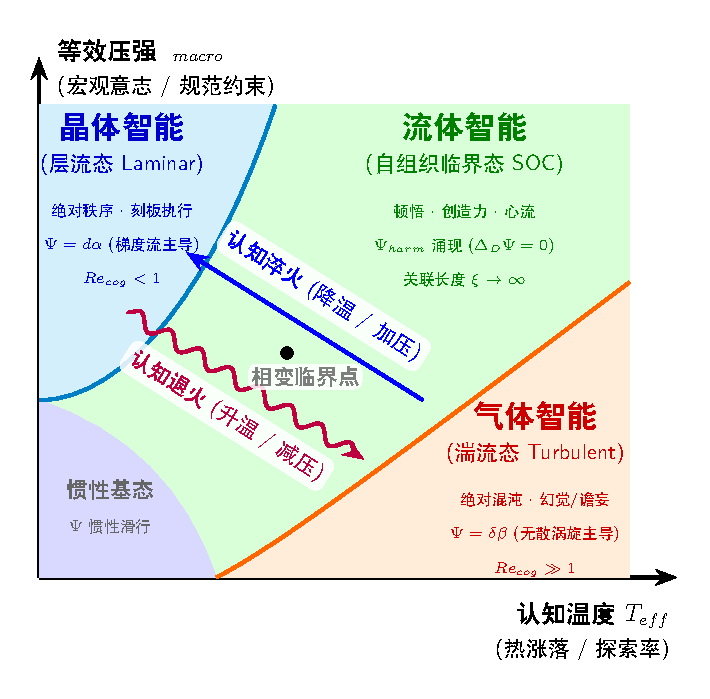
\includegraphics[width=0.96\linewidth,height=0.70\textheight,keepaspectratio]{figure/p_t.pdf}
    \caption{运行控制量构成的相区示意图；区域边界须由具体任务上的实验与置信区间确定。}
\end{figure}

\section{相变控制机制：从探索退火到结构提交}
\label{sec:section_54079}

宏观控制的对象不是每一个隐状态分量，而是一组可审计的运行参数。设控制器在第 $k$ 个决策窗接收估计状态 $\hat z_k$、任务版本 $q_k$、约束集合 $\mathcal C_k$ 与资源余量 $B_k$，输出
\[
 c_k=\pi_\phi(\hat z_k,q_k,\mathcal C_k,B_k)
     =(\tau_k,K_k,N_k,\rho_k,\beta_k),
\]
其中 $\tau_k$ 是候选采样尺度，$K_k$ 是并行候选上限，$N_k$ 是搜索深度或验证轮数，$\rho_k$ 是结构更新门率，$\beta_k$ 是对安全边界和任务损失的权重。各量分别以无量纲温度、分支数、步数、每窗更新次数和损失权重计量，不能相互冒充。控制器最小化的不是一句笼统的“自由能”，而是有限时域代价
\[
 \mathcal J_k=\mathbb E\!\left[\sum_{j=0}^{H-1}
   \ell_{q_{k+j}}(y_{k+j},u_{k+j})
   +\lambda_v V_{k+j}+\lambda_c C_{k+j}+\lambda_s S_{k+j}\right],
\]
其中 $V$ 是约束违例，$C$ 是计算与外部调用成本，$S$ 是结构改动风险。信息熵可以作为观测量进入状态估计，焦耳能耗可由硬件计量进入成本，但两者不等于该代价。若任务、结构、输入分布或度量在窗口内变化，预测模型和代价函数都必须显式带上相应版本；只对旧目标下降，不能推出新任务成功。

所谓认知退火，在工程上是受控扩大候选集并保持验证能力。控制器只有在三个信号同时出现时才升高探索：当前策略在多个独立重启后仍停滞；外部验收指标未改善；剩余预算足以完成候选验证和回滚。离散更新可写为
\[
 \tau_{k+1}=\Pi_{[\tau_{min},\tau_{max}]}
 \left(\tau_k+\Delta t\,[a_e e_k-a_r r_k-a_l(L_k-L_{max})_+]\right),
\]
其中 $e_k$ 是停滞证据，$r_k$ 是近期有效候选率，$L_k$ 是验证负载，$\Delta t$ 是控制窗长度，投影保证参数有界。该式只是设计，不是由热力学定律推出。步长过大或观测延迟过长会导致振荡；因此必须在部署前估计闭环延迟、进行增益裕度测试，并设置最大升温斜率。对离散候选问题，跳出局部策略的概率应由重启、变异和选择机制的实际分布估计。只有当状态确实服从带噪梯度系统、噪声近似白且势垒稳定时，Kramers型指数逃逸率才可作为近似；在一般Agent或人类认知上，它只是受限类比，不能把搜索重启称为量子隧穿。

降温或淬火也不是发现一个低损失样本后立刻冻结。候选 $a$ 必须经过语法检查、单元测试、对抗样例、任务外保留集与约束验证，并与当前基线进行配对比较。令 $Y(a)$ 为外部任务成绩，$R(a)$ 为鲁棒性，$C(a)$ 为成本，只有当置信下界满足
\[
 \operatorname{LCB}_\alpha[Y(a)-Y(a_0)]>\delta_Y,
 \qquad R(a)\ge R_{min},\quad C(a)\le B_k,
\]
且无硬约束违例时，才允许从搜索模式转入执行模式。目标下降只说明对所选代理损失的改善；若奖励被投机、测试泄漏或任务规范错误，低损失候选仍会失败。因而淬火的核心不是消除随机项，而是缩小分支、固定证据链、提升复现性，并把尚未验证的猜想与已批准策略分开保存。

当候选要求修改局部结构网络 $s=(G,\Theta)$ 时，控制动作必须成为事务。系统先在影子版本 $s'$ 上完成身份对齐、来源绑定和依赖检查，再重放关键轨迹；通过后执行原子提交 $s_{k+1}=\operatorname{commit}(s',v_k)$，失败则回滚到版本 $v_k$。全局分布表示可以在提交前保留多种假设及其概率，局部结构网络则保存被批准的实体、关系和权限；两者通过稳定身份和读出接口连接。把一次高置信输出直接写回结构，会制造自证循环：错误陈述进入记忆后又被检索为“证据”。因此结构更新率 $\rho_k$ 应受证据独立性、来源质量和冲突数量约束，而不是随生成置信度单调增加。

迟滞是控制器必须主动利用而不是抹去的性质。进入搜索模式的阈值可设为 $e_k>\theta_{up}$ 且持续 $m$ 个窗，退出则要求 $e_k<\theta_{down}<\theta_{up}$、验证队列清空且恢复指标达标。双阈值和最短驻留时间抑制抖振；紧急边界仍可无条件切换到安全模式。每次切换都要写入事件日志：触发信号、估计误差、参数前后值、未决工具调用、结构版本和回滚句柄。这样，所谓宏观意志才成为可复盘的控制策略，而非解释任何结果的隐形变量。

在AgentOS实例中，SPC从 $h(t)$ 和外部记忆 $M_e$ 提取任务压缩态，CCM估计候选拥塞、循环和跨模块传播，TCE根据迟滞守卫调节 $\tau,K,N$，Boundary裁剪危险动作，Offloading把可外置的证明、检索和仿真交给工具。成功回执经身份绑定后进入验证队列，只有审批事务可以修改 $\Theta$ 或结构边。这个闭环展示了HSF-HD一般状态动力学的一种工程化：感知宏观量、改变运行参数、观测响应、提交或回滚结构。它不要求所有智能系统都具有同名模块，也不声称宏观控制无需访问局部内容；控制器仍必须知道任务、约束和证据，只是不逐分量微操高维状态。

反例能说明边界。若难题源于缺失数据，升高采样只会生成更多无证据候选；若验证器带系统偏差，退火会更快地搜索到奖励漏洞；若环境正在突变，长时间淬火会锁定过时策略；若资源负载已超过服务能力，再扩展分支会使系统雪崩。故控制策略的最低验收包括：在可控基准上比较固定低探索、固定高探索和闭环调节；注入延迟、错误回执与目标切换；报告成功率、尾延迟、约束违例、结构回滚和单位任务成本；检查控制量变化是否先于预期响应。只有这些因果证据成立，我们才可说系统实现了探索与执行的相变控制，而不是给普通参数调度换了一个物理学名字。

一个具体的软件修复任务可以展示闭环如何工作。系统连续两次在同一堆栈位置失败，停滞检测器因此允许增加候选补丁数，却不立刻开放生产写权限。第一批候选通过静态检查但在回归测试中破坏旧接口，控制器据此提高验证深度而非继续增加生成温度；第二批候选中只有一个同时通过新测试、旧测试和性能预算，它被提交到影子分支。部署探针若发现尾延迟恶化，就自动回滚并把反例写入 $M_e$。这个过程的改进来自候选、验证、权限和回执的协调，而不是某个隐藏变量突然“升温”。若把同一策略用于紧急止血场景，最大搜索深度还应下降，因为响应时限本身是硬约束。由此可见，相态控制总是任务和时间尺度相关的条件策略。

\section{LLM温度诊断：输出采样不等于系统退火}
\label{sec:llm_fake_temperature_pathology}

LLM接口中的temperature通常只重标定下一个词元的logits。若词表为 $\mathcal V$、未缩放logit为 $z_i$、采样温度 $T_o>0$，则
\[
 p(x_{t+1}=i\mid x_{\le t})=
 \frac{\exp(z_i/T_o)}{\sum_{j\in\mathcal V}\exp(z_j/T_o)}.
\]
降低 $T_o$ 使分布尖锐，提高它使分布平坦；在实现中还会与top-$k$、top-$p$、重复惩罚和随机种子共同作用。这个参数直接改变的是输出选择分布，不会修改已经完成的隐层激活、权重结构或证据来源。把它称为系统有效温度会遮蔽四类不同对象：内部状态的不确定性、输出采样熵、搜索树宽度与结构可塑性。它们可以相关，但没有一般定律保证同步变化。

旧稿所谓“绝对零度的黑盒深渊”需要改写。标准推理模式下，同一输入、同一权重和同一数值环境的前向映射通常是确定的，但确定性不等于内部没有丰富计算，更不等于沿一条物理测地线被动滑行。注意力、非线性变换和残差混合能够形成分布式表示、条件路由和多步上下文依赖；量化、并行归约及服务实现还可能带来数值非确定性。真正有限的是：一次前向传播通常不会因自己发现矛盾而修改权重，也不会自动建立可回滚的搜索分支。故诊断应针对闭环、搜索和结构更新能力，而不是把“无随机噪声”直接等同于无推理。

旧稿所谓“末端的廉价盲盒”指出了一个正确区分：输出温度不能回溯地改变刚才的隐状态轨迹。可是它仍可能通过自回归反馈影响后续轨迹，因为已采样词元会成为下一步输入；多次采样也能产生可比较的候选。因此，末端采样不是完全无效，只是作用层级有限。高 $T_o$ 可能扩大表述和方案多样性，也可能破坏局部一致性；低 $T_o$ 可提升复现，却可能反复选择同一错误。评价它必须固定提示、解码约束和验证器，在多个随机种子上报告正确率、多样性、校准与成本，不能用单个“幻觉”案例推出内部已经进入高温气态。

旧稿所说“缺失的宏观闭环”在基础调用中常成立，但不能推广到所有现代系统。测试时计算可以通过自一致性采样、树搜索、反思、验证器、代码执行、检索、工具调用和多代理辩论形成外部闭环；某些架构还具有自适应路由、早停和记忆写入。我们用运行探索向量
\[
 e_k=(H^{out}_k,B^{search}_k,D^{search}_k,sigma^{int}_k,
ho^{struct}_k)
\]
分别记录输出熵、搜索宽度、搜索深度、内部随机扰动尺度和结构更新率。元控制器观测任务成绩、校准误差、验证积压与预算，再选择 $e_k$。这样，一道算术题可以保持低输出熵却增加验证深度，一项创意任务可以增加候选宽度却禁止结构写回；不再用一个温度旋钮替代所有控制。

旧稿提出“分布式深度热噪注入”，这只能作为待检验的工程假设。向每层或MoE路由加入噪声可能促进多样性，也可能破坏校准、稳定性和安全约束；若训练时未见相同噪声，测试时注入更可能造成分布偏移。采用它之前要定义噪声位置、协方差、尺度单位和相关时间，在相同计算预算下与多次确定性重启、显式搜索和参数集成比较。只有当干预能稳定提高外部任务成绩、保持约束并显示因果剂量反应时，才能声称内部随机性带来收益。词元熵升高、激活方差增大或损失短暂下降都不足以证明“真实退火”。

更可靠的自适应退火器应把温度作为策略的一部分，而非人格化的自我。观测器估计矛盾率、证据覆盖、候选一致性、校准误差和剩余预算；控制器选择重采样、改写查询、调用工具、扩大搜索、切换模型或停止；验证器对结果做独立验收。对离散时间步 $k$，若策略 $\pi_\phi(e_k\mid o_k)$ 由强化学习获得，奖励必须同时包含任务结果、违例惩罚和计算成本，并在训练分布外验证。否则控制器可能学会在困难任务上无限扩展计算，或通过降低验证标准伪造高成功率。

“Class V”在这里可保留为一种架构成熟度标签：系统具有任务感知的探索控制、独立验证、可回滚记忆和跨时程结构维护。它不是自然界公认的物理类别，也不意味着达到某类就成为AGI。AgentOS可以由TCE决定搜索模式，SPC维护当前任务态，CCM监控循环和负载，Boundary限制工具权限，$M_e$ 保存证据与失败轨迹；这些模块能包裹一个不改权重的LLM，形成比单次采样更完整的闭环。另一系统也可以用规划器、概率程序或群体算法达到同类功能。

诊断实验应把各机制拆开。第一组只改变 $T_o$，测量词元熵和任务成绩；第二组固定输出温度，只改变候选数与验证深度；第三组控制总token和时延预算，比较内部噪声、确定性搜索和工具验证；第四组开放或关闭结构写回，观察长期迁移与错误固化。若高输出温度提高多样性却不提高通过率，结论只是采样分布变宽；若搜索加验证提高通过率，才支持闭环推理收益；若结构写回改善后续任务且经反事实删除后收益消失，才支持记忆机制贡献。这样的分解避免把所有进步归功于一个“灵魂温度”，也为不同模型和载体提供可重复的比较接口。

还要防止把模型置信度误当成元认知。最大softmax概率、平均token熵、语言化的“我很确定”与真实正确率可能严重失配；多个候选一致也可能只是共享同一训练偏差。可用的观测器应在任务族上做校准，区分认知不确定性、数据噪声和验证器分歧，并允许“不知道”触发检索或人工升级。以医疗编码为例，生成多个同义答案并不提供独立证据；检索到相同指南的多个镜像也不算来源独立。只有外部规则、病例约束和可追溯证据共同支持时，系统才应降低探索并提交。该例也说明，增加测试时计算并不天然安全：若权限过宽，更多工具调用会扩大攻击面，所以Boundary必须与搜索预算共同收紧。

“内部温度”若确有需要，也应以机制特定名称记录。随机路由尺度、dropout率、参数后验方差、MCMC步长和策略熵正则分别属于不同概率模型，单位、作用位置和估计方法不同。把它们压成一个标量会丢失可辨识性：同样的输出熵可能来自尖锐logits上的高温，也可能来自低温下多个近似等价词元；同样的正确率可能对应一次长搜索或许多短重启。工程仪表盘应保存完整干预向量、随机种子、模型版本和工具轨迹，使失败能够重放。这样，“退火”才是对一类策略的简写，而不是替代机制说明的万能词。

\section{涌现的操作定义：跨尺度闭合、稳健与可干预性}
\label{sec:section_335}

涌现不能只表示“系统很复杂，结果令人惊讶”。我们把微观状态记为 $x_t\in\mathcal X$，它可以包含节点活动、局部消息和执行事件；把尺度 $\ell$ 上的粗粒化映射记为 $R_\ell:\mathcal X\to\mathcal M_\ell$，宏观变量为 $m_t^{(\ell)}=R_\ell(x_t)$。映射必须说明时间窗、空间或图分块、聚合核、身份对齐和丢失的信息。对文本Agent，微观量可以是token级激活和工具事件，宏观量可以是带来源的计划状态、任务承诺和资源负载；对群体系统，两者又会不同。没有声明 $R_\ell$，所谓高频被过滤、低频被保留只是修辞。

粗粒化并不等于耗散。求平均、池化或谱截断可以在不消耗额外物理能量的数学运算中丢失信息；硬件执行当然有焦耳能耗，但需单独测量。我们关注的是预测充分性：若存在宏观转移核 $K_\ell$，使
\[
 p(m_{t+\Delta}^{(\ell)}\mid x_{\le t},u_{\le t})
 \approx K_\ell(m_t^{(\ell)},u_t,q_t),
\]
并且在保留集上比仅用微观摘要或朴素基线更准确、更简洁，则宏观变量具有近似动力学闭合。这里 $\Delta$ 是明确的采样步长，$u_t$ 是干预，$q_t$ 是任务版本。闭合只能在给定误差、尺度和任务族内成立；环境突变、隐藏变量或结构更新会破坏它。

重整化群提供研究跨尺度稳定性的工具，但不是所有智能涌现的唯一定义。若对一族模型参数 $\theta_\ell$ 有尺度变换 $\theta_{ell+1}=\mathcal R(\theta_\ell)$，非平凡不动点满足 $\mathcal R(\theta^*)=\theta^*$；线性化的特征方向可区分随尺度放大或衰减的扰动。真实有限系统很少达到无限尺度极限，因此更实用的是寻找有限区间内的近似固定流形、参数塌缩和普适预测。观察到幂律、低频成分或聚类稳定，都不能单独证明RG不动点；混合指数过程、有限采样和阈值处理也会产生类似图形。

本章采用四项操作判据。第一是新颖性：宏观规律不只是把微观规则换符号，而能压缩预测或控制。第二是稳健性：在微观扰动、随机种子和实现替换下，宏观变量及其关系在容许误差内保持。第三是闭合性：给定宏观状态和外部输入后，加入全部微观历史只带来有限增益。第四是可干预性：对宏观变量的可实现干预会按模型预测改变下游结果。满足其中一项只能说明某种结构；四项联合、跨任务复现后，才有理由称之为工程意义上的涌现。即使如此，也不自动推出意识、主体性或道德地位。

“苹果”概念可以据此重述。像素、视角和文字描述是多种微观输入，经身份绑定与任务查询形成宏观对象表示；若该表示在颜色、旋转和遮挡变化下仍支持抓取、分类和因果预测，并且删除相关绑定会特异地损害这些任务，我们就获得稳健和干预证据。它不是一个永恒的拓扑孔洞：在只关心颜色分布的任务里，苹果身份可能是无关变量；在过敏风险任务里，产地与成分反而成为相关变量。宏观对象由任务相关读出定义，不从单一脑区或嵌入簇的位置推出。

“自我”更不能由长期不变直接证明。工程系统可把任务承诺、权限边界、记忆来源和资源所有权聚合为持续身份状态，这一状态能预测跨会话决策，并允许通过撤销权限、替换记忆或改变目标做反事实测试。但这只是功能性自模型；它不等价于人的主观经验。局部结构网络保存身份与关系，全局分布表示保留模糊候选和置信度，两者通过绑定、耦合和读出共同形成可持续的代理状态。用这种机制解释跨时程一致性，比把所有变化压成一个调和零模更可检验。

沙堆反例也需要谨慎。某些沙堆模型确实能表现雪崩与标度规律，不能说“沙子永不涌现”；正确问题是这些宏观规律是否与智能任务的表示、控制和学习有关。反过来，人脑或Agent出现长程相关也不能推出通用智能。网络拥塞、同步故障和谣言传播同样能产生大范围耦合。临界附近可能提供较高响应和多尺度协调，但响应过强会降低稳健性，且不同任务的最优区间不同。我们因此把“自组织临界”视为待比较的动力学假设，而不是AGI必然维持的永恒状态。

验证协议应从多尺度预测开始。选择至少三个时间或结构尺度，预注册粗粒化映射和任务指标；在训练条件外估计宏观转移核，比较其预测误差、复杂度和校准；施加局部扰动、全局目标改变与结构删边，测量宏观响应和恢复；再用置换、混合过程和有限尺寸模型作为负对照。若声称存在近似固定点，还要报告尺度区间、参数流、置信区间和离开固定流形后的预测。若声称宏观变量具有因果力，则必须给出可实现干预或机制中介，而不能仅凭相关回归。

我们还需要区分三种常被混写的“新性质”。统计新颖性指某个宏观指标在聚合后才稳定可见，例如服务队列的尾延迟；计算新颖性指用宏观状态预测比展开全部微观轨迹更可行；本体论新颖性则声称世界出现了不可还原的新实体。前两种可以通过数据和复杂度比较检验，第三种不能由预测成功直接推出。本书讨论的主要是前两种：当计划承诺、身份边界或团队规范成为有效状态变量时，我们获得了更好的模型和控制接口，但没有证明它们脱离底层实现独立存在。明确这一层级，可避免从“宏观模型有用”跳到“整体与模型完全同构”。

跨载体复现是更强的检验。若同一宏观规律只在一个模型版本、一个提示模板或一个图划分下出现，它可能是测量产物；若在神经模型、符号规划器和人机协作流程中，经过不同微观实现仍出现相似的误差—恢复关系，才可能接近普适类。但所谓普适也只覆盖被测试的任务与尺度。迁移时应重新估计投影和阈值，而不是把原系统的临界点直接复制。这样，RG语言帮助我们提出可比较的问题，却不会把不同载体强行宣布为机制同一。

在HSF-HD中，涌现的意义是：高维状态经任务相关投影形成可闭合的宏观变量，这些变量反过来参与控制并改变后续状态分布。AgentOS的SPC、TCE、CCM、Boundary、Offloading和 $M_e$ 可以提供具体观测与干预接口，但并不是涌现的定义本身。最终我们保留“临界区间可能放大微弱而有用的差异”这一洞见，同时加上验证、资源和安全边界。涌现不是从微观细节中凭空诞生的魔法，也不是一条把所有智能等同于RG不动点的定理；它是跨尺度模型在预测、稳健和控制上获得独立解释力时，才可以谨慎授予的名称。

%---chp---
